\documentclass[10pt,a4paper]{article}
\usepackage[T1]{fontenc}
\usepackage[utf8]{inputenc}
\usepackage{lmodern}
\usepackage[margin=0.72in]{geometry}
\usepackage{setspace}
\usepackage{graphicx}
\usepackage{booktabs}
\usepackage{array}
\usepackage{tabularx}
\usepackage{amsmath}
\usepackage{microtype}
\usepackage{xcolor}
\usepackage{caption}
\usepackage{subcaption}
\usepackage{enumitem}
\usepackage{float}
\usepackage[hidelinks]{hyperref}
\setstretch{1.04}
\setlist{nosep,leftmargin=*}
\captionsetup{font=small,labelfont=bf,skip=3pt}
\renewcommand{\arraystretch}{1.12}
\setlength{\parindent}{0pt}
\setlength{\parskip}{3.5pt}
\setcounter{secnumdepth}{2}

\begin{document}

\begin{center}
{\large\bfseries Military Institute of Science and Technology\par}
\vspace{0.05in}
{\normalsize\bfseries Department of Computer Science and Engineering\par}
\vspace{0.12in}
\rule{\textwidth}{0.5pt}\par
\vspace{0.10in}
{\LARGE\bfseries A Learned Selector for Classical Disk Scheduling\par}
\vspace{0.07in}
{\large Term Paper -- Track 2\par}
\vspace{0.13in}
\begin{tabularx}{0.90\textwidth}{@{}>{\bfseries\raggedright\arraybackslash}p{1.25in} >{\raggedright\arraybackslash}X
                                      >{\bfseries\raggedright\arraybackslash}p{0.90in} >{\raggedright\arraybackslash}p{1.15in}@{}}
Student Name: & Aria Nawshin Ashka & Student ID: & 202414021 \\
Course: & CSE-307 & Course Title: & Operating Systems \\
\end{tabularx}
\vspace{0.08in}
\rule{\textwidth}{0.5pt}
\end{center}
\vspace{-0.04in}

\begin{abstract}
No fixed disk-scheduling policy is optimal for every request pattern. This work implements FCFS, SSTF, SCAN, and C-SCAN and trains a small decision tree to choose a policy from an incoming request window. Experiments use reproducible sequential, random, and bursty synthetic workloads, disjoint training, validation, and test seeds, and explicit workload shifts. On 660 held-out 50-request windows, the main selector achieved 75.61\% tie-aware accuracy and 124,574 tracks of movement, improving on the best fixed policy, SSTF (133,276), while approaching an offline oracle (119,296). Confidence was higher on correct than incorrect predictions (0.877 versus 0.778), although an expected calibration error (ECE) of 0.148 shows overconfidence remains. A validation-selected random-forest extension improved accuracy and calibration but not seek regret, demonstrating why decision accuracy and operating-system cost must both be reported.
\end{abstract}

\noindent\textbf{Keywords:} disk scheduling, FCFS, SSTF, SCAN, C-SCAN, decision tree, calibration

\section{Introduction and System Design}
Disk scheduling determines the order in which a device services pending track requests. FCFS preserves arrival order but can travel unnecessarily; SSTF greedily chooses the nearest request and may starve distant requests; SCAN sweeps like an elevator; and C-SCAN provides a one-directional sweep with a wrap \cite{osc}. Their relative cost depends on locality and request order, motivating an adaptive selector.

The simulator uses tracks 0--199. In the main experiment the head resets to 50 for every independent, non-overlapping 50-request window. Following the course convention, SCAN initially moves toward 0, reaches physical track 0, then reverses. C-SCAN also moves toward 0, reaches 0, wraps to 199, and counts that wrap. Unit tests reproduce the course queue $[98,183,37,122,14,124,65,67]$ from head 53: FCFS=640, SSTF=236, SCAN=236, and C-SCAN=386.

For each window, all four algorithms run offline. The minimum-cost algorithm is the oracle label. All tied winners are stored; exact ties are excluded only from primary classifier fitting. The main classifier is an interpretable decision tree (depth 5, minimum leaf size 12, balanced class weights, fixed seed), a standard classification method \cite{cart}. It receives eight pre-decision features: variance, range, mean absolute consecutive gap, gap coefficient of variation, direction consistency, mean distance from the head, and fractions below and above the head. Confidence is the maximum predicted class probability.

\section{Experimental Method}
Sequential workloads are mostly monotonic with small positional noise; random workloads are uniform over all tracks; and bursty workloads contain ordered clusters around several hot spots. Twenty windows per workload are generated for every seed. Seeds 1--20 train the model, 21--30 form a validation set, and 100--110 are held out for final testing. This yields 1,200 training and 660 test windows. The training set contains 63 unique FCFS, 267 SCAN, and 800 SSTF labels, plus 70 ties. C-SCAN never uniquely wins.

Two 40-window stress timelines change after window 20: sequential$\rightarrow$random and random$\rightarrow$bursty. Metrics are total seek, tie-aware accuracy, selector regret (selected cost minus oracle cost), confusion matrix, confidence on correct versus wrong cases, a reliability diagram, and 10-bin ECE \cite{calibration}. The implementation uses Python, NumPy, pandas, Matplotlib, and scikit-learn \cite{sklearn}; raw CSVs and fixed seeds make every result reproducible.

\begin{table}[H]
\centering
\caption{Total seek on all 660 held-out windows. ``Always SSTF'' is the strongest single fixed-policy baseline.}
\label{tab:overall}
\small
\begin{tabular}{lr@{\qquad}lr}
\toprule
Policy & Total seek & Policy & Total seek \\
\midrule
FCFS & 902,104 & C-SCAN & 251,307 \\
Always SSTF & 133,276 & Oracle & 119,296 \\
SCAN & 144,737 & Learned selector & \textbf{124,574} \\
\bottomrule
\end{tabular}
\end{table}

\section{Results and Analysis}
Table~\ref{tab:overall} shows that the selector saves 8,702 tracks (6.53\%) relative to always choosing SSTF. It is only 5,278 tracks above the oracle over all windows, or 8.00 tracks per window. The 597 non-tied windows give 74.37\% ordinary accuracy; accepting any tied oracle winner gives 75.61\% over all 660 windows. Classification accuracy alone is insufficient: a wrong choice may have almost the same seek cost as the winner, while a less frequent error can be expensive.

\begin{table}[H]
\centering
\caption{Per-workload held-out seek totals for 220 windows each.}
\label{tab:workload}
\scriptsize
\begin{tabular}{lrrrrrrr}
\toprule
Workload & FCFS & SSTF & SCAN & C-SCAN & Oracle & Selector & Acc. \\
\midrule
Sequential & 44,549 & 38,504 & 46,291 & 84,450 & 35,020 & 39,214 & 62.7\% \\
Random & 729,441 & 63,558 & 54,054 & 86,664 & 53,398 & 54,098 & 70.9\% \\
Bursty & 128,114 & 31,214 & 44,392 & 80,193 & 30,878 & 31,262 & 93.2\% \\
\bottomrule
\end{tabular}
\end{table}

Table~\ref{tab:workload} exposes the main weakness rather than hiding it. Sequential accuracy is only 62.7\%, with mean regret 19.06, compared with 3.18 for random and 1.75 for bursty workloads. The confusion matrix in Fig.~\ref{fig:diagnostics} shows most errors involve SSTF versus FCFS or SCAN. Nevertheless, the selector nearly matches the oracle on random and bursty workloads.

C-SCAN never wins under this experimental convention because the head begins near the lower end (50), movement is initially toward 0, and the complete 0$\rightarrow$199 wrap is charged. That fixed wrap is expensive for these finite windows. This is a result of the stated geometry and cost model, not a claim that C-SCAN is universally inferior; fairness and starvation are not included in the objective.

Confidence is meaningfully informative: the main tree averages 0.877 when correct and 0.778 when wrong. However, ECE=0.148 and the reliability curve show imperfect calibration. Under the sequential$\rightarrow$random shift, mean regret falls from 19.06 to 3.18 after the change while confidence falls from 0.861 to 0.809. Under random$\rightarrow$bursty, regret falls from 4.32 to 1.49 and confidence rises from 0.799 to 0.889. Thus the model responds to changed feature distributions, but its probability should not be interpreted as a guarantee.

\begin{figure}[H]
\centering
\begin{subfigure}{0.49\textwidth}
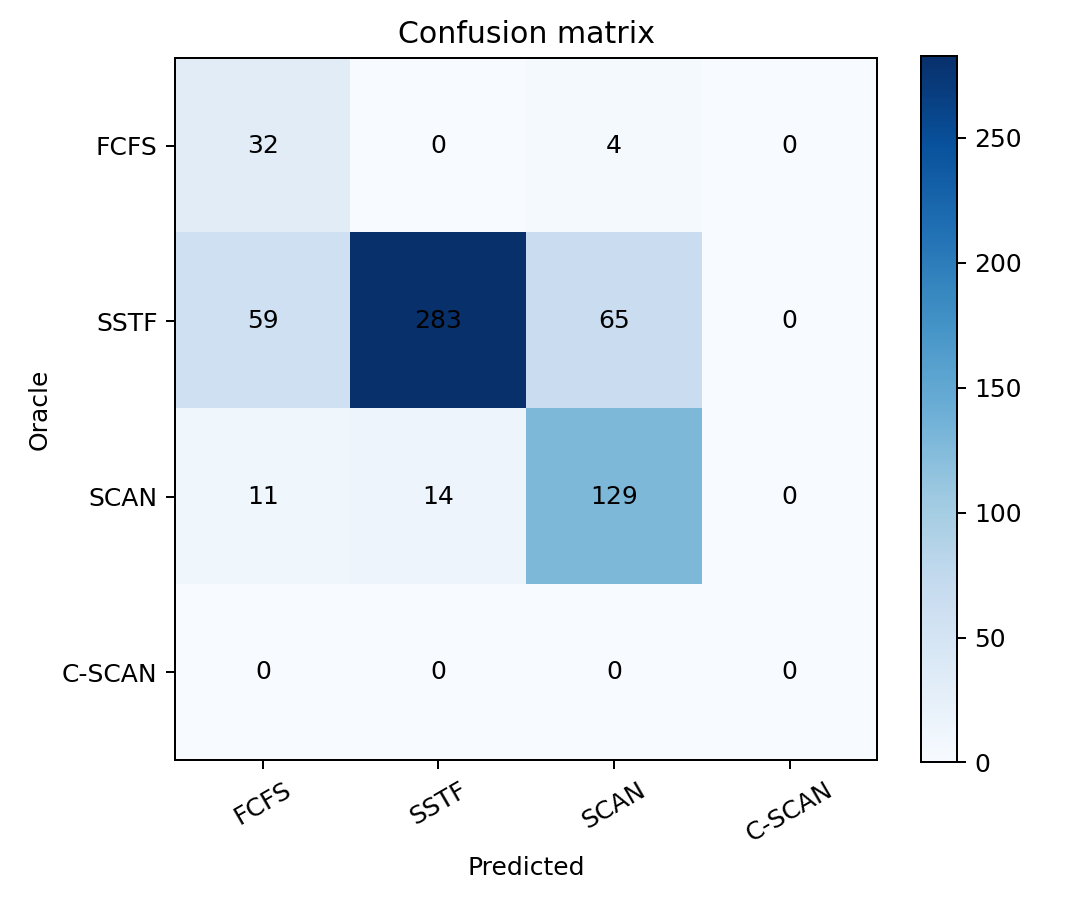
\includegraphics[width=\linewidth]{../results/confusion_matrix.png}
\caption{Non-tied confusion matrix.}
\end{subfigure}\hfill
\begin{subfigure}{0.49\textwidth}
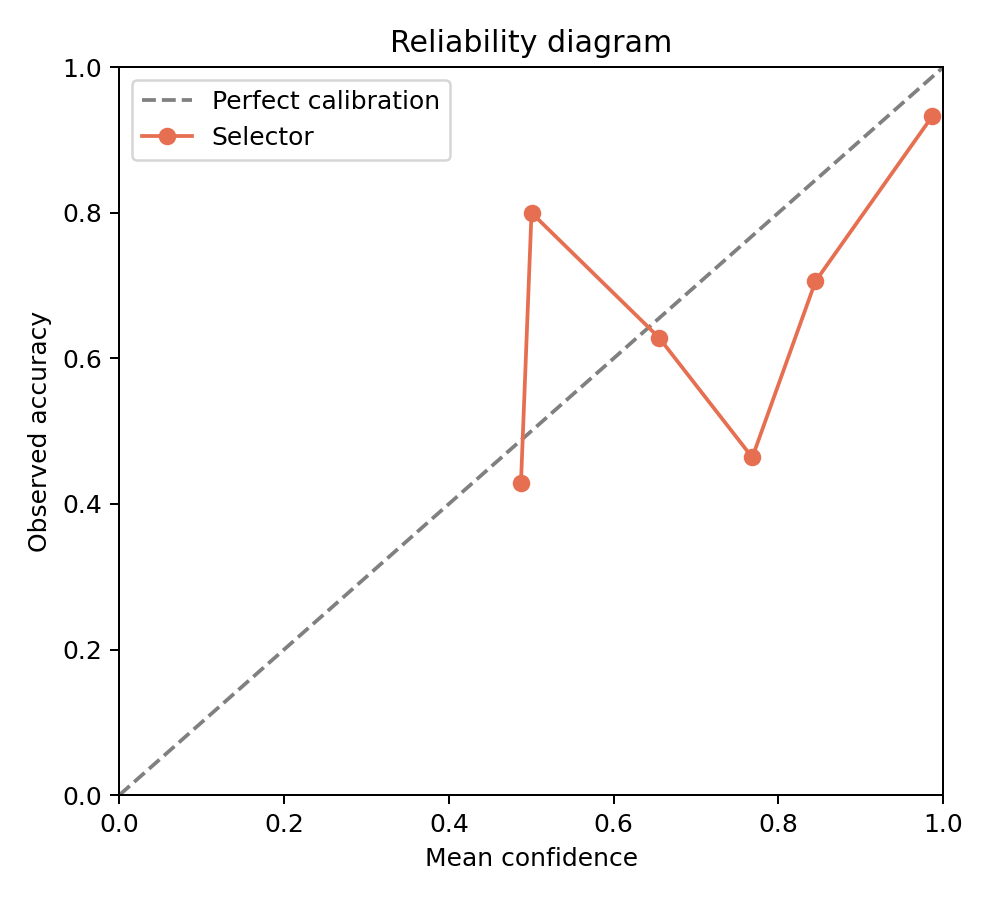
\includegraphics[width=\linewidth]{../results/calibration_reliability.png}
\caption{Reliability diagram.}
\end{subfigure}
\caption{Diagnostic evidence for classification and confidence.}
\label{fig:diagnostics}
\end{figure}

\section{Validation-Controlled Extensions}
Four additional features target sequential structure: absolute correlation between request index and track, fraction of consecutive gaps at most five, median gap, and maximum gap. A logistic-regression baseline and a 300-tree random forest were trained on seeds 1--20. Model choice used only validation seeds 21--30; the random forest won with 78.5\% validation accuracy and ECE 0.028. It was then evaluated once on the held-out test set.

The forest reaches 79.09\% tie-aware test accuracy, 70.91\% sequential accuracy, and ECE 0.051; confidence separates correct and wrong predictions more clearly (0.827 versus 0.615). Yet its mean regret is 8.90 and total seek is 125,170, slightly worse than the main tree. Logistic regression is weaker at 73.33\% accuracy and 10.44 mean regret. Therefore the tree remains the primary result: it is simpler to explain and minimizes the measured seek objective, while the forest is a useful calibration-focused extension.

A window-size sensitivity check retrains the tree at 30, 50, and 100 requests. Tie-aware accuracy is 81.52\%, 75.61\%, and 84.39\%, respectively; mean regret is 4.05, 8.00, and 2.95. SSTF remains the best fixed scheduler at each size, and the selector remains better than that fixed baseline. The exact performance is sensitive to window length, but the principal ranking is unchanged.

\section{Limitations and Conclusion}
This simulation measures seek distance only. It omits rotational latency, caching, SSD behavior, concurrent arrivals during service, priorities, starvation, and device-level timing. Complete windows and an offline oracle simplify a real online problem. The fixed head and fixed SCAN direction also limit generalization. Future work should use rolling windows, multiple head positions, cost-sensitive training, and calibration learned on a dedicated calibration set.

Within these limits, the learned tree improves over every fixed scheduler and comes close to the oracle while exposing useful confidence information. The results also show an important systems lesson: the most accurate classifier need not minimize operational cost. All code, seeds, raw outputs, figures, tests, and an interactive custom-queue demonstration are included for audit and reproduction.

\subsection*{AI-Use Disclosure}
Generative AI assisted with scaffolding, implementation, documentation, and debugging. All numerical claims in this paper were regenerated by deterministic code and checked against committed CSV/JSON outputs. The student remains responsible for understanding and defending the work.

\begin{thebibliography}{9}\small
\bibitem{osc} A. Silberschatz, P. B. Galvin, and G. Gagne, \emph{Operating System Concepts}, 10th ed., Wiley, 2018.
\bibitem{cart} L. Breiman, J. H. Friedman, R. A. Olshen, and C. J. Stone, \emph{Classification and Regression Trees}. Wadsworth, 1984.
\bibitem{calibration} C. Guo, G. Pleiss, Y. Sun, and K. Q. Weinberger, ``On Calibration of Modern Neural Networks,'' in \emph{Proc. ICML}, 2017, pp. 1321--1330.
\bibitem{sklearn} F. Pedregosa et al., ``Scikit-learn: Machine Learning in Python,'' \emph{JMLR}, vol. 12, pp. 2825--2830, 2011.
\end{thebibliography}

\end{document}

